\section{Zielsetzung}
\label{sec:Ziel}
In diesem Versuch wird die Funktionsweise und charakteristische Eigenschaften eines \textit{Geiger-Müller-Zählrohrs} untersucht. Dabei wird die Länge des Plateubereiches
und die Totzeit des Zählrohres ermittelt.

\section{Theorie}
\label{sec:Theorie}
Das Geiger-Müller-Zählrohr wird verwendet um Strahlungsintensitäten ionisierender Strahlung zu messen. Prinzipiell ionisieren die einfallenden Teilchen (oder Lichtquanten) der 
$\alpha$-, $\beta$- oder $\gamma$-Strahlung Atome im Inneren des Zählrohres, was zu einem elektrischen Signal führt. Die genaue Funktionsweise des Geiger-Müller-Zählrohres
--auch \textit{GMZ} genannt-- wird im Folgenden beschrieben.

\subsection{Funktionsweise eines Geiger-Müller-Zählrohres}
\label{subsec:Funktion_GMZ}
Das \textit{GMZ} besteht im Wesentlichen aus einer zylinderförmigen Kathode, in dessen Zentrum ein Anodendraht verläuft. Wie die Benennung bereits suggeriert, wird eine Spannung 
an die beiden Bauteile angelegt. An der Vorderseite der Apparatur befindetr sich ein Eintrittsfenster aus Mylar, welches auch das Eindringen von leicht zu absorbierender
Strahlung (wie $\alpha$-Strahlung) ermöglicht. Der Innenraum des Zählrohres ist mit einem Gas (\textit{Zählgas}) gefüllt, welches mit Alkoholdämpfen versetzt ist. Auf die Funktion
letzterer wird später eingegangen.
Der beschriebene Aufbau des \textit{GMZ} ist in \autoref{fig:GMZ_Aufbau} dargestellt. Die Polung der anliegenden Spannung ist ebenfalls der Abbildung zu entnehmen.

\begin{figure}
    \centering
    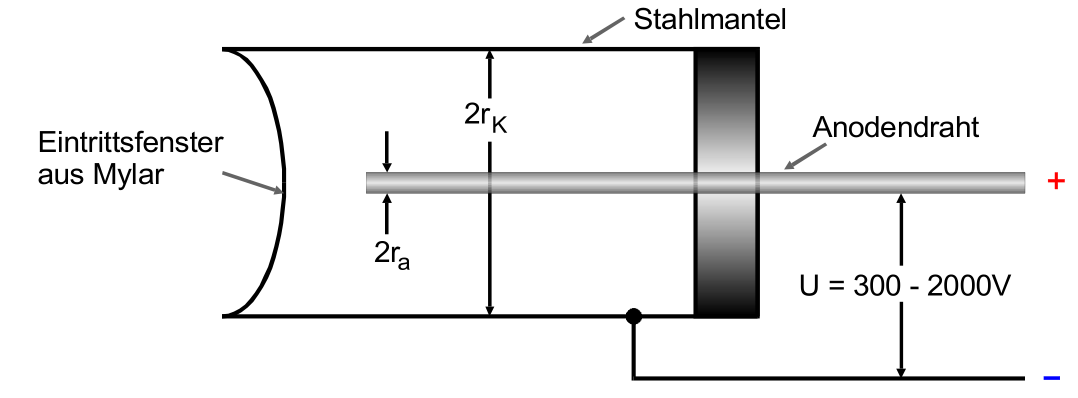
\includegraphics[width = .8\textwidth]{content/GMZ_Aufbau.png}
    \caption{Aufbau eines Geiger-Müller-Zählrohres \cite{v703}.}
    \label{fig:GMZ_Aufbau}
  \end{figure}

Wie oben bereits erwähnt, kommt es durch einfallende Strahlung zu Ionisation von Gasmolekülen. Da es vor der Absorption des Teilchens zu einer Vielzahl von Ionisationsakten
kommt, bei welchen im Mittel eine Energie von nur $\qty{26}{\electronvolt}$ abgegeben wird, ist die Anzahl der ionisierten Teilchen proportional zur Energie der Strahlung.

Die nun separierten Elektronen-Ionen Paare bewegen sich anschließend auf Grund der anliegenden Spannung in Richtung der Anode bzw. Kathode. Dabei treten abhängig von der 
Spannung verschiedene Prozesse auf. Es lassen sich verschiedene Bereiche identifizieren, die in \autoref{fig:Bereiche} eingetragen sind.

\begin{figure}
  \centering
  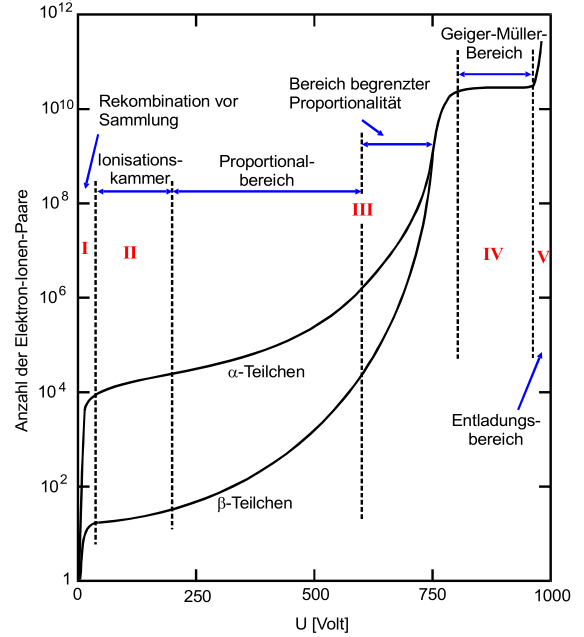
\includegraphics[width = .5\textwidth]{content/Bereiche.png}
  \caption{Anzahl der Ionenpaare gegen die Spannung und Unterteilung in verschiedene Bereiche \cite{v703}.}
  \label{fig:Bereiche}
\end{figure}

\begin{description}
  \item[1) Rekombination]\hfill \\
    Ein Großteil der ionisierten Teilchen rekombiniert wieder zu neutralen Teilchen, da die Beschleunigungsspannung zwischen Anode und Kathode zu gering ist.
  \item[2) Ionisationskammer]\hfill \\
    Die Ionisationskammer ist eine Vorstufe zum Zählrohr. In diesem Bereich gelangen praktisch alle Elektronen zum Anodendraht. Der so entstehende Strom ist 
    sehr gering und proportional zur Energie und zur Intensität der Strahlung.
  \item[3) Proportionalbereich]\hfill \\
    Im Proportionalbereich erlangen die beschleunigten Elektronen soviel Energie, dass sie selbst wieder Moleküle/Atome ionisieren können. Es entsteht eine
    Elektronenlawine, die sogenannte \textit{Townsend-Lawine}. Es sammelt sich eine ausreichend Große Menge an Ladung an, sodass Ladungsimpulse, die proportional
    zur Energie der Strahlung sind, gemessen werden können. Ein Detektor, welcher in diesem Bereich arbeitet wird Proportionalzählrohr genannt. Mit einem solchen
    Zählrohr können Strahlungsintensitäten und -Energien gemessen werden.
  \item[4) Geiger-Müller-Bereich]\hfill \\   
    In diesem Bereich kommt zu Elektronenlawinen im ganzen Volumen des Zählrohres, welche durch UV-Photonen aus der primären Elektronenlawine ausgelöst werden. 
    Da so die Proportionalität zur Primärionisation verloren geht, kann nur noch auf die Strahlungsintensität geschlossen werden. Pro einfallendem Teilchen sammelt 
    sich genügend Ladung an um diese auf einfache Weise nachweisen zu können. Dies ist der Funktionsbereich des \textit{GMZ}.
  \item[5) Entladungsbereich]\hfill \\
    Im Entladungsbereich erreichen die Ionen eine Energie, die es ihnen ermöglicht Elektronen aus dem Kathodenmantel auszulösen (\textit{Sekundärelektronen}). 
    Dieser Prozess wird \textit{Nachentladung} genannt und kann durch wiederholte Kettenreaktionen zu einer Dauerentladung führen, was hohe Stromdichten bedingt 
    und somit zur Zerstörung des Zählrohres führt. Nachentladungsprozesse treten auch im Geiger-Müller-Bereich auf, weshalb Alkoholmoleküle dem Gasgemisch 
    des \textit{GMZ} hinzugefügt werden, welche durch Kollision mit den Edelgasionen die Nachentladung verhindern sollen.
\end{description}

Der Anodenstrom ist offensichtlich proportional zur freigesetzten Ladungsmenge ($I = \dot{Q}$). Sein Mittelwert kann mithilfe der in der Zeit $\symup{\Delta}t$ registrierten
Teilchenzahl $Z$ und der pro Zeiteinheit transportierten Ladungsmenge $\symup{\Delta}Q$ über 
\begin{equation}
  \label{eqn:Strom}
  \overline{I} = \frac{\symup{\Delta}Q}{\symup{\Delta}t}Z
\end{equation} 
berechnet werden.
\subsection{Tot- und Erholungszeit eines Zählrohres}
\label{subsec:Totzeit}
Aufgrund der im Vergleich zu den Elektronen großen Masse der positiven Ionen bewegen sich diese langsamer zur Kathode. Es entsteht eine positive Raumladung 
(\textit{Ionenschlauch}), der das elektrische Feld zwischen Anodendraht und Kathode abschwächt. Dies hat zur Folge, dass für eine Zeit $T$ keine Stoßionisation
stattfinden kann und somit keine Elektronenlawinen gebildet werden können. Strahlung, welche in dieser Zeit in das Geiger-Müller-Zählrohr eindringt, kann also
nicht detektiert werden. Die Zeit $T$ wird Totzeit genannt. Sobald die positive Ladungswolke zur Kathode abwandert, steigt die effektive Feldstärke wieder an 
und es können wieder Elektronenlawinen entstehen. Die Zeit, bis alle Ionen wieder neutralisiert sind wird Erholungszeit $T_\text{E}$ genannt.

\subsection{Charakteristik eines Geiger-Müller-Zählrohres}
\label{subsec:Charakteristik}
Durch Auftragen der gemessenen Teilchenzahl $N$ gegen die Spannung $U$ zwischen Kathode und Anode entsteht bei konstanter Strahlungsintensität eine Kurve, die
die Charakteristik eines Geiger-Müller-Zählrohres beschreibt. Eine solche Kurve ist in \autoref{fig:Charakteristik} dargestellt. Der gezeigte Bereich entspricht
dem Bereich 4) aus \autoref{fig:Bereiche}.

\begin{figure}
  \centering
  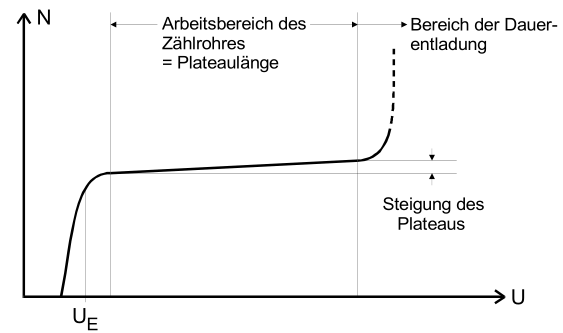
\includegraphics[width = .7\textwidth]{content/Charakteristik.png}
  \caption{Charakteristische Kurve eines Geiger-Müller-Zählrohres \cite{v703}.}
  \label{fig:Charakteristik}
\end{figure}

Der Bereich der linearen Steigung wird \textit{Plateau} genannt. Er ist der Arbeitsbereich des Zählrohres. Seine Länge und Steigung sind ein Maß 
für die Qualität des Messinstrumentes. Dabei sollte die Länge möglichst groß und der Anstieg möglichst gering ausfallen. Die Steigung wird üblicherweise
pro $\qty{100}{\volt}$ angegeben und wird durch Nachentladungen verursacht, die trotz des Alkoholzusatzes entstehen.
